\documentclass[12pt]{article}

%%%%%%%%%%%%PACKAGES%%%%%%%%%%%%%%
\usepackage[top=2cm,bottom=2cm, right = 1cm, left = 1.5cm]{geometry}
\usepackage{fancyhdr}

\usepackage[T2A]{fontenc}
\usepackage[english, russian]{babel}
\usepackage{tempora}% bold titles and nice style
\usepackage{graphicx}%%%allow inserting images
\usepackage{xcolor}
\usepackage{enumitem}
\usepackage{float}
%%%%%%%%%%%%%%%%%%%%%%%%%%%%%%%%%

%%%%%%%%%%%%%%%%%%%%%%%%%%preambules%%%%%%%%%%%%%%%%%%%%
%%%%%%%%%%%%%%%%%%%%%%%%%%%%%%%%%%%%%%%%%%%%%%%%%%%%%%%%

\pagestyle{fancy}
\fancyhead{}
\fancyfoot{}%clear all the footnotes
\fancyhead[L]{\slshape\MakeUppercase{Django Installation}}
\fancyhead[R]{\slshape{Neder Mendez}}
\fancyfoot[C]{\thepage}%set the notes as the page number
\setlength{\parskip}{0.5em} %lenght between paragrahs
\renewcommand{\baselinestretch}{1.2}%spacing between lines
\parindent 0ex %remove the espace of the first line in every paragraph

%%%%%%%%%%%%%%%%%%%%%%%%%%custom colors%%%%%%%%%%%%%%%%%%%%%%%%%%
%%%%%%%%%%%%%%%%%%%%%%%%%%%%%%%%%%%%%%%%%%%%%%%%%%%%

\usepackage{listings}
\definecolor{codegreen}{rgb}{0.1,0.7,0.1}
\definecolor{codegray}{rgb}{0.5,0.5,0.5}
\definecolor{codepurple}{rgb}{0.7,0,0.98}
\definecolor{codemagenta}{rgb}{1,0,1}
\definecolor{backcolour}{rgb}{1,1,1}
\definecolor{aqua}{rgb}{0.0, 1.0, 1.0}
\definecolor{myyellow}{rgb}{0.9, 0.9, 0.0}

%%%%%%%%%%%%%%%%%%%%%%%%%listing styles%%%%%%%%%%%%%%%%%%%%%%%%%%
%%%%%%%%%%%%%%%%%%%%%%%%%%%%%%%%%%%%%%%%%%%%%%%%%%%%

\usepackage{listings}

\lstdefinestyle{conlst}{
	morekeywords={[1] .py},
	keywordstyle={ [1]\color{orange} },
	basicstyle=\Large\ttfamily,
	commentstyle=\color{gray} \emph,
	stringstyle=\ttfamily,
	numbers=left,
	numberstyle=\small, 
	stepnumber=1, 
	numbersep=5pt,
	backgroundcolor=\color{backcolour},
	stringstyle=\color{codegreen},
	showspaces=false,
	showtabs=false,
	breaklines=true,
	showstringspaces=false,
	breakatwhitespace=true,
	upquote=true,
	frame=tblr,
	escapechar =@,
	columns=fullflexible
	%aboveskip=20pt,
	%belowskip=20pt
	}

\lstdefinestyle{pylst}{
	language=Python,
	morekeywords={[1] None, True, False},
	morekeywords={[2] __init__, __name__},
	morekeywords={[3] self},
	basicstyle=\Large\ttfamily,
	keywordstyle={[1]\color{blue}},
	keywordstyle={[2]\color{codemagenta}},
	keywordstyle={[3]\color{codepurple}},
	keywordstyle={[4]\color{codegreen}},
	commentstyle=\color{codegreen} \emph,
	%stringstyle=\ttfamily,
	numbers=left,
	numberstyle=\small, 
	stepnumber=1, 
	numbersep=5pt,
	backgroundcolor=\color{backcolour},
	stringstyle=\color{orange},
	showspaces=false,
	showtabs=false,
	breaklines=true,
	showstringspaces=false,
	breakatwhitespace=true,
	upquote=true,
	frame=tblr,
	escapechar =@,
	columns=fullflexible,
	%aboveskip=20pt,
	%belowskip=20pt
	}

\lstset{literate=%
   *{0}{{{\color{codegreen}0}}}1
    {1}{{{\color{codegreen}1}}}1
    {2}{{{\color{codegreen}2}}}1
    {3}{{{\color{codegreen}3}}}1
    {4}{{{\color{codegreen}4}}}1
    {5}{{{\color{codegreen}5}}}1
    {6}{{{\color{codegreen}6}}}1
    {7}{{{\color{codegreen}7}}}1
    {8}{{{\color{codegreen}8}}}1
    {9}{{{\color{codegreen}9}}}1
}

%%%%%%%%%%%%%%%%%%%%%%%%%%%%%%%%%%%%%%%%%%%%%%%%%%%%%%%%%%
%%%%%%%%%%%%%%%%%%%%%%%%%%%%%%%%%%%%%%%%%%%%%%%%%%%%%%%%%%

\begin{document}
\setcounter{page}{1}%set this page as the first page

\section{Check if python is already installed}\label{sec:check}
\begin{itemize}
	\item  {Open the windows console pressing the keys: \texttt{windows(windows key) + r}. Then write \texttt{cmd} and press \texttt{ok}.

	      \begin{figure}[H]
		      \centering
		      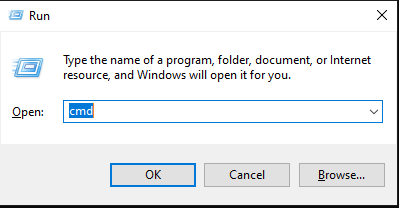
\includegraphics[width =0.7\textwidth ,keepaspectratio]{imgs/open_console.png}
		      \caption{}
	      \end{figure}
	      }

	\item  {Write the next command in console:

	      \begin{lstlisting}[caption=\phantom{},style=conlst,label={check_version}]
python --version
\end{lstlisting}

	      \begin{figure}[H]
		      \centering
		      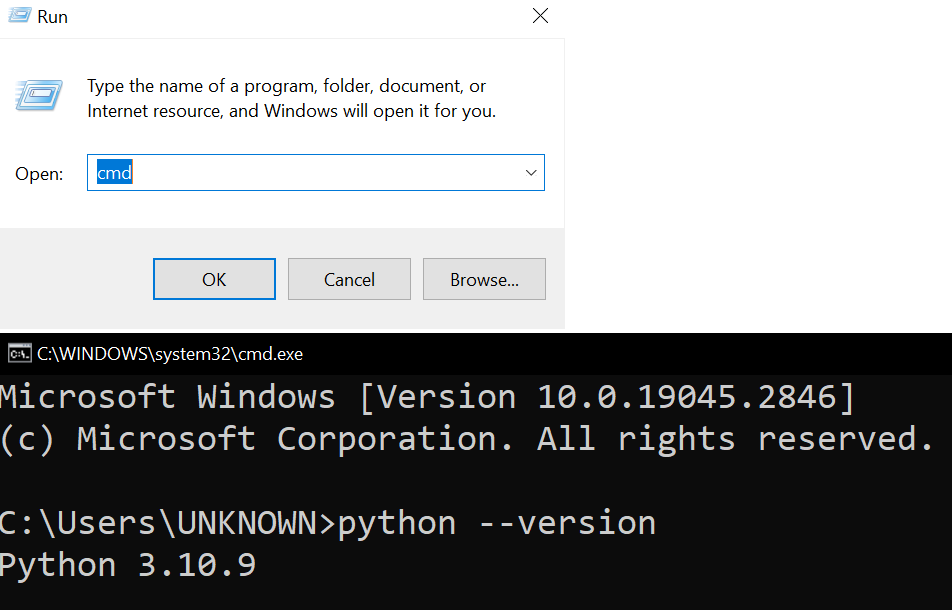
\includegraphics[width =0.7\textwidth ,keepaspectratio]{imgs/check_python.png}
		      \caption{}
	      \end{figure}

	      }
\end{itemize}

If the command of the listing \ref{check_version} returns a valid version then you already have python installed.
However if no version is shown then you need to install python following the next steps.

\section{Install Python}

To install python go to the search bar and write \emph{store} then open the microsoft store and type in the search bar \emph{python},
then click on get . Is recommended to dowload the version \texttt{3.10}.

\begin{figure}[H]
	\centering
	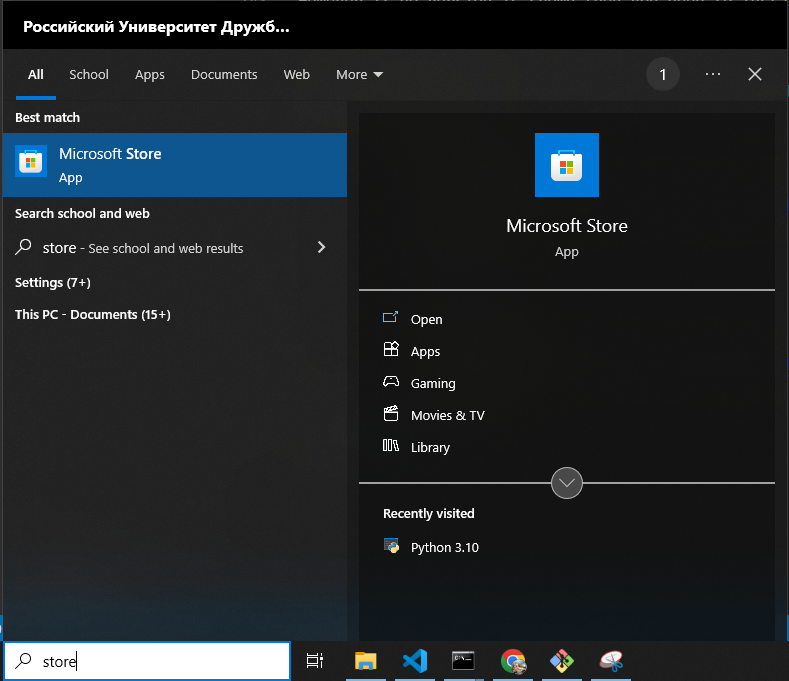
\includegraphics[width=0.5\textwidth ,keepaspectratio]{imgs/open_store.png}
	\caption{}
\end{figure}


\begin{figure}[H]
	\centering
	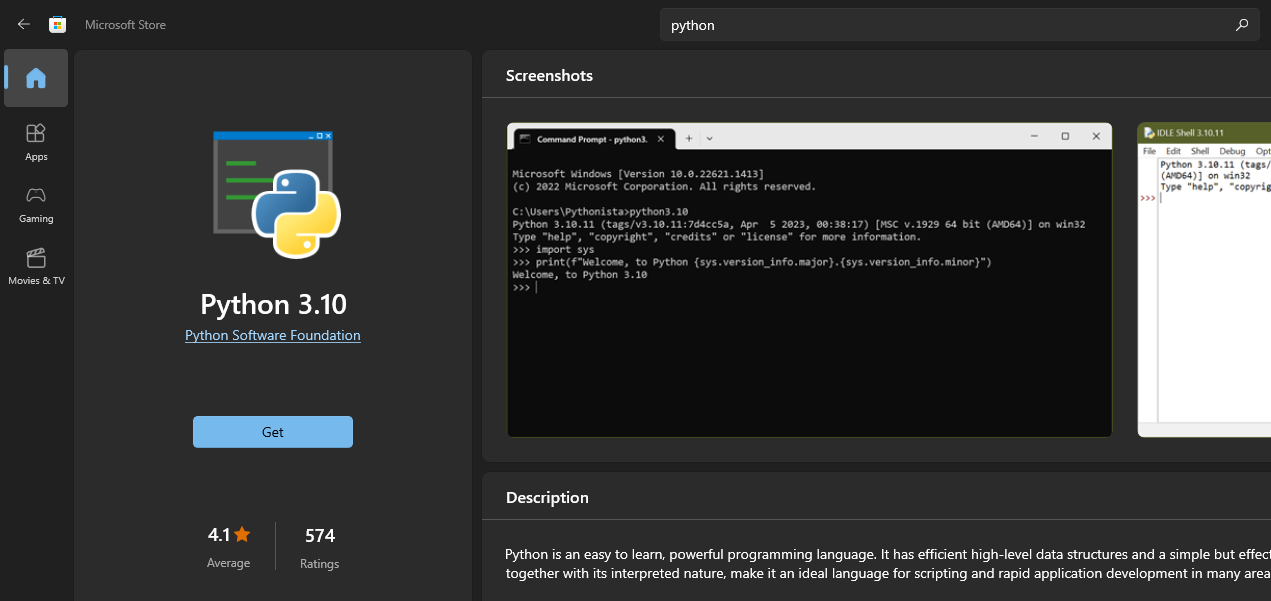
\includegraphics[width =1\textwidth ,keepaspectratio]{imgs/install_from_store.png}
	\caption{}
\end{figure}

After installing python, try again the steps shown in the section \ref{check_version} and check the version is shown.
\end{document}